\documentclass{article}
\title{PHYS114 Reference}
\author{Krish A. Patel}

\usepackage{amsmath}
\usepackage{graphicx}
\usepackage{indentfirst}
\usepackage{tikz}
\usetikzlibrary{calc}

\newcommand{\vsp}{\vspace{1em}}
\newcommand{\rect}{\text{rect}}
\newcommand{\sinc}{\text{sinc}}
\renewcommand{\arraystretch}{1.5}

\tikzset{
    block/.style={draw, rectangle, minimum width=2cm, minimum height=1.5cm, thick, text centered},
    arr/.style={->, >=stealth, thick}
}

\begin{document}

\maketitle
\input{notes/data_software_figs}
\input{notes/research_intro}
\input{notes/fwd_model_photometer}
\input{notes/dist_err_analysis}
\section{Remote Sensing}

\textbf{Remote sensing} is the science of obtaining information about objects or areas from a distance, typically from aircraft or satellites. \textbf{Passive} remote sensing "watches" the system, collecting without impacting the system (e.g., photometer). \textbf{Active} remote sensing perturbs the system until it reaches steady-state again (e.g., radar). This "nudge" must be small to minimize disruption to the system. Passive remote sensing equipment is preferred as it tends to be less complex than active remote sensing equipment.

\subsection{LiDAR}

LiDAR, which stands for Light Detection and Ranging, is an active remote sensing method that uses pulses of infrared (or sometimes visible or ultraviolet) light to measure the system. LiDAR offers a higher resolution than radar due to using shorter wavelength of light than radio waves.

\subsection{Radar}

Radar, which stands for Radio Detection and Ranging, is an active remote sensing method that uses radio waves to measure the system. Radar offers a lower resolution than LiDAR due to using radio waves, which have a longer wavelength.

\subsection{Angle of Spread}

\begin{align*}
    \theta & \sim \frac{\lambda}{D}                                 \\
    \theta & = 1.22 \frac{\lambda}{D} \tag*{for circular apertures}
\end{align*}

where
\begin{itemize}
    \item $\theta$ is the angle of spread,
    \item $\lambda$ is the wavelength of the light,
    \item $D$ is the diameter of the aperture.
\end{itemize}

Thus it is clear why radar has a lower resolution than LiDAR, because radio waves have a longer wavelength and thus spread out much more. This leads to a \textbf{volume underfilled} scenario, in which the target does not fill the entire volume of the beam.

\subsection{Doppler Effect}

\begin{align*}
    \lambda' & = \frac{v - v_s}{f}                 \\
    f'       & = f_0'(\frac{v \pm v_o}{v \mp v_s})
\end{align*}

where
\begin{itemize}
    \item $\lambda'$ is the observed shifted wavelength,
    \item $f'$ is the observed shifted frequency,
    \item $v$ is the speed of the wave,
    \item $v_o$ is the speed of the observer,
    \item $v_s$ is the speed of the source, and
    \item $f_0'$ is the emitted frequency.
\end{itemize}

\textbf{Sign conventions}: In the numerator, use + if the observer is moving towards the source, and - if the observer is moving away from the source. In the denominator, use - if the source is moving towards the observer, and + if the source is moving away from the observer.

\subsection{Monostatic and Bistatic Systems}

In a \textbf{monostatic} system, the transmitter and receiver are at the same location. In a \textbf{bistatic} system, the transmitter and receiver are at different locations (usually common for speed detection in rural areas).

\subsection{Speed Detection}

Speed detection is a common application of remote sensing and can use either radar or LiDAR. Radar speed detection uses the doppler effect to measure the speed of a vehicle, whereas LiDAR speed detection uses the time it takes for the light to return to the sensor to calculate the vehicle's speed.

Radar has a low \textbf{signal-to-noise ratio} (SNR) compared to LiDAR at the receiver, allowing a car to detect when its speed is being tracked and jamming the reflected signal (thus, radio detectors have been outlawed in many places). LiDAR has a high SNR (especially when directed at license plates with a special coating), so while a car still detect when its speed is being tracked, it cannot jam the reflected signal (as a result, LiDAR detectors have not been outlawed).

\subsection{Stealth}

Stealth aircraft conceal themselves to radar detection by using a combination of radar-absorbent materials and clever geometry to deflect radar waves away from the receiver. This is why stealth aircraft are not completely invisible to radar, but they have a very low radar cross-section.

\subsection{Jenny Jump}

Jenny Jump uses active remote sensing to detect the height that particles are in the atmosphere. The transmitter sends a beam of green light up into the atmosphere 30 times per second. (One pulse would have a low SNR, which is solved by stacking 30 pulses.) The receiver then detects the light that is scattered back to it from the particles in the atmosphere. The height of the particles is then calculated using the time it takes for the light to return to the receiver:

\begin{align*}
    z = \frac{c \Delta t}{2}
\end{align*}

Among other information, this receiver can detect gravity waves (which are a type of buoyancy waves) in the atmosphere. Gravity waves are a cause of clear-air turbulence, which is a hazard for aircraft.
\section{Monte Carlo Methods}

This class does not focus on Monte Carlo methods, but here is a brief overview. \textbf{Monte Carlo methods} are a broad class of computational algorithms that rely on repeated random sampling to estimate possible outcomes of complex, uncertain events. Random number generation is a complex topic, yet it is important for simulations. For example, the simulation of light scattering and weather models predicting a hurricane's path use Monte Carlo methods. Weather models are \textbf{ensemble models}, which means that they run the same simulation multiple times with different initial conditions to generate a range of possible outcomes and account for uncertainty. Ensemble models only help for so long until the models start diverging greatly.
\section{Fitting Simple Curves}

\subsection{Straight Line}

Forward model:

\begin{equation*}
    y = a_0 + b_0 x
\end{equation*}

Let $\sigma_i$ denote the uncertainty in $y_i$. (The uncertainty in $x_i$ is assumed to be 0.) $x_i$ and $y_i$ are the data points.

Minimize $\Delta y = y_i - y(x_i)$, the difference between the data points and the model. Assume that each $y_i$ is pulled from a stationary Gaussian distribution, and use the maximum likelihood method.

The probability of a particular observation is
\begin{equation*}
    P_i = \frac{1}{\sigma_i \sqrt{2\pi}} \exp\left[-\frac{1}{2}\left(\frac{y_i - y(x_i)}{\sigma_i}\right)^2\right]\text{.}
\end{equation*}

For $N$ measurements:

\begin{equation*}
    \prod_{i=1}^{N} P_i = \prod_{i=1}^{N}\left(\frac{1}{ \sigma_i \sqrt{2\pi}}\right) \exp\left[-\frac{1}{2}\sum_{i=1}^{N}\left(\frac{y_i - y(x_i)}{\sigma_i}\right)^2\right]\text{.}
\end{equation*}

For the model $y = a_0 + b_0 x$:

\begin{equation*}
    P(a_0, b_0) = \prod_{i=1}^{N}\left(\frac{1}{ \sigma_i \sqrt{2\pi}}\right) \exp\left[-\frac{1}{2}\sum_{i=1}^{N}\left(\frac{y_i - (a_0 + b_0 x_i)}{\sigma_i}\right)^2\right]
\end{equation*}

To maximize $P(a_0, b_0)$, we need to minimize the exponent:

\begin{equation*}
    \chi^2 = \sum_{i=1}^{N}\left(\frac{y_i - (a_0 + b_0 x_i)}{\sigma_i}\right)^2
\end{equation*}

To minimize $\chi^2$, we take the partial derivatives with respect to $a_0$ and $b_0$ and set them to 0.

\vsp
\begin{equation*}
    \frac{\partial \chi^2}{\partial a_0} = 0 \quad \text{and} \quad \frac{\partial \chi^2}{\partial b_0} = 0\text{.}
\end{equation*}

The result is:

\begin{align*}
    \Delta = \sum \frac{1}{\sigma_i^2} \sum \frac{x_i^2}{\sigma_i^2} - \left(\sum \frac{x_i}{\sigma_i^2}\right)^2                                             \\
    a_0 = \frac{1}{\Delta} \left( \sum \frac{x_i^2}{\sigma_i^2} \sum \frac{y_i}{\sigma_i^2} - \sum \frac{x_i}{\sigma_i^2} \sum \frac{y_i}{\sigma_i^2} \right) \\
\end{align*}

$b_0$ can be found as well, but the formula is not the focus of this course.
\vsp
The unertainty on $a_0$ and $b_0$ is given by:
\begin{align*}
    \sigma_z^2 = \sum \sigma_i^2 \left(\frac{\partial z}{\partial y_i}\right)^2
\end{align*}

where $z$ can be $a_0$ or $b_0$. Note that the number of contraints $n_C$ is 2 since due to $a_0$ and $b_0$.

\subsection{Polynomials}

Forward model:

\begin{equation*}
    y(x_i) = \sum_{k=1}^m a_k f_k(x_i)
\end{equation*}

where $f_k(x_i) = 1, x_i, x_i^2, \dots$ is a polynomial parent function.

\vsp
Carry out a similar process as fitting a straight line:

\begin{equation*}
    P = \prod_{i=1}^{N}\left(\frac{1}{ \sigma_i \sqrt{2\pi}}\right) \exp\left[-\frac{1}{2}\sum_{i=1}^{N}\left(\frac{y_i - \sum_{k=1}^m a_k f_k(x_i)}{\sigma_i}\right)^2\right]
\end{equation*}

Thus:

\begin{equation*}
    \frac{\partial \chi^2}{\partial a_\ell} = 0 \tag*{for $\ell = 1, \dots, m$}
\end{equation*}
\section{Linearization}

Linearization is the process of transforming a non-linear function into a linear function:

\begin{align*}
    y &= Ae^{-bx}           \\
    \ln y &= \ln (Ae^{-bx}) \\
    \ln y &= \ln A - bx
\end{align*}
\section{System Theory}

\textbf{System theory} is the study of how individual components of a system interact with each other to produce a collective behavior. A \textbf{linear time-invariant (LTI)} system is a system that satisfies the following properties:
\begin{itemize}
    \item \textbf{Linearity}: If the input is multiplied by a constant, the output is multiplied by the same constant.
    \item \textbf{Time-invariance}: If the input is shifted in time, the output is shifted by the same amount of time. In other words, the time at which the input is provided does not affect the system's output.
\end{itemize}

A simple diagram of a system is:
\begin{center}
    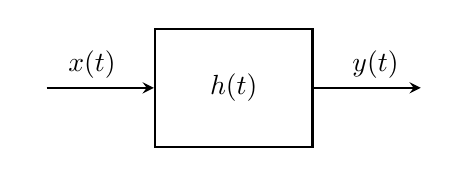
\begin{tikzpicture}
        % Input coordinate and label
        \node (input) at (0,0) {};
        \node [above] at (0.7,0) {$x(t)$};

        % The System Block
        \node [block] (system) at (2.5,0) {$h(t)$};

        % Output coordinate and label
        \node (output) at (5,0) {};
        \node [above] at (4.3,0) {$y(t)$};

        % Arrows
        \draw [->, >=stealth, thick] (input) -- (system);
        \draw [->, >=stealth, thick] (system) -- (output);
    \end{tikzpicture}
\end{center}

where $x(t)$ is the input, $h(t)$ is the system, and $y(t)$ is the output. The system is often considered a "black box" meaning we can only infer the properties of the system by observing the input and output.

\vsp
A system can also have a feedback from the output to the input, represented by $f(x)$:

\begin{center}
    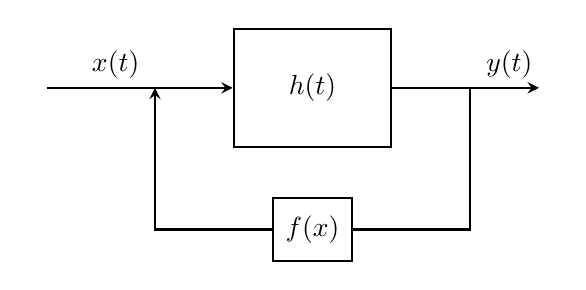
\begin{tikzpicture}[fblock/.style={draw, rectangle, minimum width=1cm, minimum height=0.8cm, thick, text centered}]
        % --- Nodes ---
        \node [block] (system) at (2.5, 0) {$h(t)$};
        \node (input)  at (-1, 0) {};
        \node (output) at (5.5, 0) {};

        % --- Main Flow ---
        \draw [arr] (input) -- (system);
        \draw [arr] (system) -- (output);

        % --- Labels ---
        \node [above] at (0, 0) {$x(t)$};
        \node [above] at (5, 0) {$y(t)$};

        % --- Feedback Loop with Function Block ---
        \node [fblock] (feedback) at (2.5, -1.8) {$f(x)$};

        \draw [thick] (4.5, 0) |- (feedback);
        \draw [arr] (feedback) -| (0.5, 0);

    \end{tikzpicture}
\end{center}

System theory involving feedback is called \textbf{control theory}.
\section{Perturbation Theory}

The notation from system theory carries over:
\begin{itemize}
    \item $x(t)$ is the input
    \item $y(t)$ is the output
    \item $h(t)$ is the system
\end{itemize}

\subsection{Dirac-Delta Function}

\begin{align*}
    \delta(t)                            & \equiv \begin{cases} \infty & t = 0 \\ 0 & t \neq 0 \end{cases} \\
    \int_{-\infty}^{\infty} \delta(t) dt & = 1
\end{align*}

The Dirac-Delta function is continuous, which is useful in analog applications.

\subsection{Kronecker Delta Function}

\begin{align*}
    \delta_{ij} & \equiv \begin{cases} 1 & i = j \\ 0 & i \neq j \end{cases}
\end{align*}

The Kronecker Delta function is discrete, which is useful in digital applications such as digital signal processing (DSP).

\subsection{Step Function}

\begin{align*}
    u(t)              & \equiv \begin{cases} 1 & t \ge 0 \\ 0 & t < 0 \end{cases} \\
    \frac{d}{dt} u(t) & = \delta(t)
\end{align*}

Also known as the Heaviside step function.

\subsection{Rectangle Function}

\begin{align*}
    \rect\left(\frac{t - t_0}{a}\right) & \equiv (\text{a rectangle centered at $x=t_0$ with width $a$}) \\
    \rect\left(\frac{t - X}{Y}\right)   & \equiv u(t - X + Y/2) - u(t - X - Y/2)
\end{align*}

\subsection{Sinc Function}

\begin{align*}
    \sinc(x) & \equiv \frac{\sin x}{x}
\end{align*}

\subsection{Convolutions}

To get the output from the input:
\begin{equation*}
    y(t) = x(t) \ast h(t)
\end{equation*}

where $\ast$ is the convolution operator, defined as:
\begin{equation*}
    x(t) \ast h(t) = \int_{-\infty}^{\infty} x(\tau) h(t - \tau) d\tau
\end{equation*}

Convolutions can be informally thought as "smearing" two things together. Convolutions can be computed mathematically or graphically. In this class, we will only compute convolutions graphically.

Properties:
\begin{itemize}
    \item When $x(t) = \delta(t)$, $y(t) = h(t)$.
    \item After many convolutions, the output will approach a Gaussian distribution.
    \item A delay circuit is when a function is shifted without distortion.
\end{itemize}
\section{Fourier Transform}

\begin{equation*}
    \mathcal{F}\left\{x(t)\right\} \equiv X(\omega) \equiv \int_{-\infty}^{\infty} x(t) e^{-i\omega t} dt
\end{equation*}

The \textbf{Fourier transform} $\mathcal{F}$ maps a signal from the time domain to the frequency ($\omega$) domain. It can also be used on spatial data. A key advantage of the Fourier transform is data compression: frequency values often take up much less storage space than a full representation of the signal in the time domain.

\vsp
The convention is to use a lowercase function like $x(t)$ in the time domain and an uppercase function like $X(\omega)$ in the frequency domain.

\vsp
The integral usually yields a real and an imaginary component. The imaginary component contains phase information. However, we are usually only interested in the real component since that yields frequency information.

\subsection{Discrete Fourier Transform}

\begin{equation*}
    \mathcal{F}\left\{x(n)\right\} \equiv X(k) \equiv \sum_{n = 0}^{N-1} x(n) e^{-i\frac{2\pi kn}{N}}
\end{equation*}

where $N$ is the number of data points.

\vsp
The \textbf{discrete Fourier transform (DFT)} is suitable for computers. However, in practice, software uses the FFT.

\subsection{Fast Fourier Transform}

If $N = 2^q$ for some integer $q$, then the DFT can be computed much faster using the \textbf{fast Fourier transform (FFT)}. Whereas the regular Fourier transform and DFT take $O(N^2)$ time to compute, the FFT takes $O(N \log N)$ time to compute. Any number of data points can be brought to the next highest power of 2 by padding the ends with zeros (a technique called \textbf{zero-padding}).

\subsection{Fourier Transform Table}

There are many Fourier transform pairs, but these are the ones we will need in this class.

\begin{table}[h]
    \centering
    \begin{tabular}{cc}
        $x(t)$              & $X(\omega)$                                                    \\
        \hline
        \hline
        1                   & $2\pi \delta(\omega)$                                          \\
        $\delta(t)$         & 1                                                              \\
        $\rect(t/T)$        & $T ~ \sinc(\frac{T}{2\pi} \omega)$                             \\
        $\sinc(\omega t)$   & $\frac{1}{\omega_0} \rect(\frac{\omega}{2\pi \omega_0})$       \\
        $\cos (\omega_0 t)$ & $\pi[\delta(\omega - \omega_0) + \delta(\omega + \omega_0)]$   \\
        $\sin (\omega_0 t)$ & $-i\pi[\delta(\omega - \omega_0) - \delta(\omega + \omega_0)]$ \\
        \hline
    \end{tabular}
\end{table}

\subsection{Convolution Theorem}

\begin{equation*}
    x(t) \ast h(t) = \mathcal{F}^{-1}\left\{\mathcal{F}\left\{x(t)\right\} \mathcal{F}\left\{h(t)\right\}\right\}
\end{equation*}
Notice that multiplication in the time domain is equivalent to convolution in the frequency domain, and convolution in the time domain is equivalent to multiplication in the frequency domain.

This theorem is useful in because convolutions are much slower to compute than the Fourier transform.

\subsection{PSD}

[work in progress - this topic will be covered later in the class]

\begin{equation*}
    \text{PSD}(\omega) = \left| X(\omega) \right|^2 = (\text{real})^2
\end{equation*}

\subsection{Windowing Functions}

The Fourier transform inherently messes with the spectral content of a signal. To mitigate this, we can use windowing functions.

\begin{equation*}
    \mathcal{F}\left\{x(t)\right\} = \mathcal{F}\left\{x(t)w(t)\right\} = X(\omega) \ast W(\omega)
\end{equation*}

where $w(t)$ is the windowing function.

The perfect window needs an infinite number of data points, which is impossible to achieve in practice. Instead, we want to minimize the \textbf{width} of the \textbf{main lobe} in a dB-vs-frequency plot of the window function.

\subsubsection{Hanning Window}

\begin{equation*}
    W(n) = \frac{1}{2}\left[1 - \cos\left(\frac{2\pi n}{N-1}\right)\right]
\end{equation*}

PSD has multiple full-forms:

\begin{itemize}
    \item Power Spectrum
    \item Power Spectrum Distribution
    \item Power Spectral Distribution
    \item Power Spectral Density
\end{itemize}

Each are technically defined differently, but are often used interchangeably. We will stick to PSD to avoid any confusion.
\end{document}
